% 黒魔術
\expandafter\ifx\csname ifdraft\endcsname\relax
    \documentclass[a4paper,twoside,12pt,papersize, dvipdfmx]{iirthesis}
    \usepackage{amsmath,amssymb,amsthm}
    \usepackage{graphicx}
    \usepackage{subcaption}
    \usepackage{url}
    \usepackage{otf}
    \usepackage{minitoc}
    \usepackage{bm}
    \usepackage{amsmath,amssymb}
    \begin{document}

    \newcommand{\figref}[1]{\figurename\ref{#1}}
    \newcommand{\tabref}[1]{\tablename\ref{#1}}
    \renewcommand{\eqref}[1]{式~(\ref{#1})}
    \newcommand{\chapref}[1]{\ref{#1}章}
    \newcommand{\secref}[1]{\ref{#1}節}
    \newcommand{\ssecref}[1]{\ref{#1}項}
    \newcommand{\appref}[1]{付録\ref{#1}}
\fi


\chapter{序論}\label{chap::intro}
\minitoc

\section{研究背景}\label{sec::intro::background}
人間が物を扱う中で日常的に行っている動作として,「In-handマニピュレーション」というものがある.これは手の中で物体の位置や向きを変化させる動作のことで,例えば,机の上のスマートフォンを持ち上げ,操作しやすいように手の中でスマートフォンを持ち替える動作に該当する.このIn-handマニピュレーションをロボットハンドで実現しようとした研究は数多く存在する(\figref{fig::intro::ihm}).現状,これらの研究の多くは,対象物とロボットハンドの接触位置や接触力,摩擦力を考慮した複雑な制御のもと実現されている.また外乱に対して脆弱であり,センサの誤作動や外部環境の影響で失敗する場合が多い.\par

ところで,対象物の拘束手法の一つにケージング\cite{rimon1999}というものがある.これは,対象物の形状情報を基に,ロボットハンドによる幾何学的な囲い込みで対象物を拘束する手法である.この手法では,ロボットハンドの位置制御のみで実現可能であり,モデルが単純かつセンサを必要としない.また外乱にも強く,例えば対象物に力が加わり移動したとしても,ロボットハンドの囲い内にあれば拘束は継続される. \par

\begin{figure}[b]
\centering
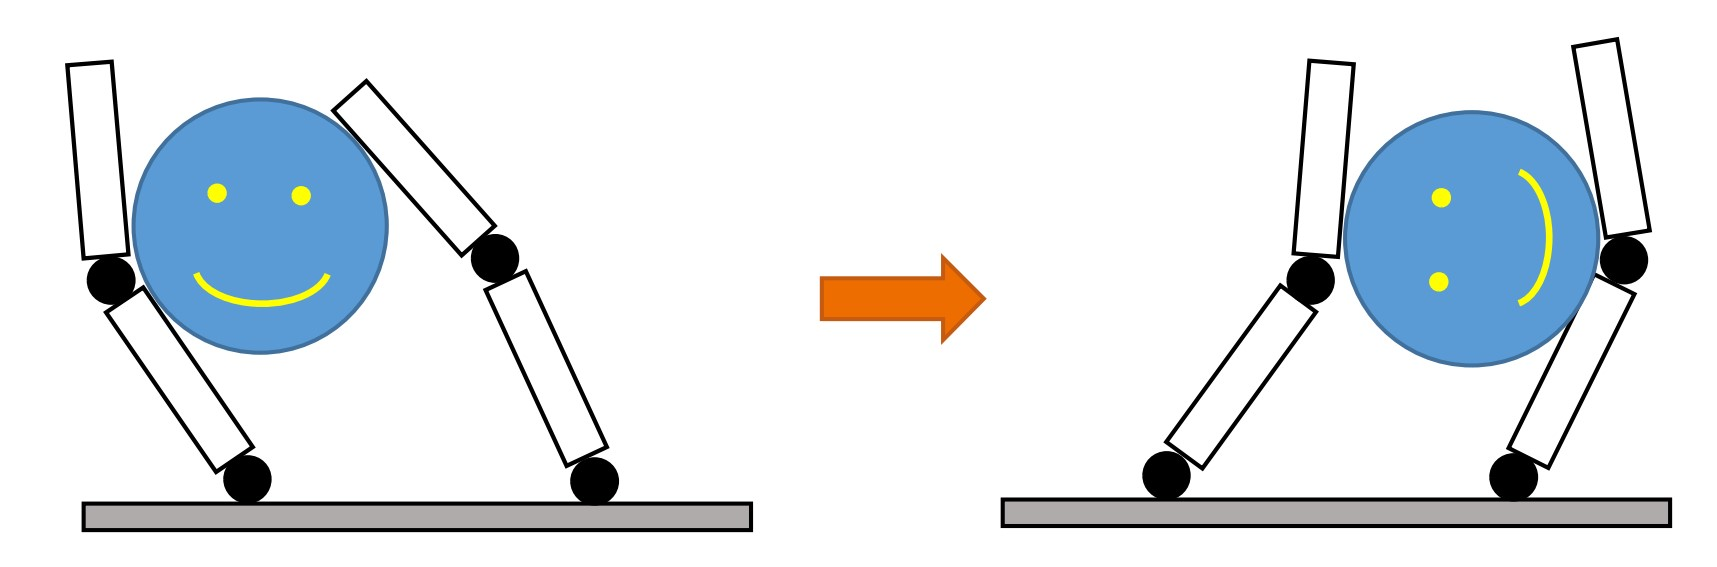
\includegraphics[width=0.7\hsize]{fig/1-introduction/in-hand.jpg}
\caption{In-hand manipulation by a robot hand \cite{komiyama2021}}
\label{fig::intro::ihm}
\end{figure}

ケージングを用いることで,外界センサを使わないIn-handマニピュレーションを実現できる.具体的には,ロボットハンドで対象物をケージングにより拘束した後,囲いの形状を変化させていくことで,対象物の位置・姿勢(傾き)を操ることができる.\cite{komiyama2021}では,これを「センサレスin-handケージングマニピュレーション」と定義している.外界センサを使わないため安価にシステムを構築でき,またロボットハンドの位置情報のみを取り扱うのでシンプルな制御で事足りる.また,ケージングは外乱に強いため,本マニピュレーション手法においても,その恩恵を受け,外乱に強くなる可能性がある.

本手法は,位置・姿勢(傾き)にばらつきのある対象物を特定の位置・姿勢に整列できるという特徴を踏まえて,工場の製造ライン等で用いられるパーツフィーダとして応用できると考えられる.昨今,日本では労働力不足に伴い自動化の需要が増してきている.しかし,通常,部品整列で使われるパーツフィーダ専用機や産業用ロボットを用いたパーツフィーダシステムは導入コストが高く,小規模な工場等では導入が進んでいない.一方,本手法は外界センサを一切使わないためコストが低い.また,後述するが本手法は多様な形状の対象物をマニピュレーションできるため,多品種少量生産にある昨今に有用で導入しやすいパーツフィーダになると考えられる.


\section{従来研究}\label{sec::intro::relatedresearch}
\subsection{In-handマニピュレーションに関する研究}
\subsubsection{Planning In-hand Object Manipulation with Multifingered Hands Considering Task Constraints \cite{hertkorn2013}}
この研究では,人間の指のような多自由度のハンドを用いた,3次元の物体のin-handマニピュレーション問題を扱っている.物体は,ハンドと物体との接触(Force closure)によって把持されている.対象物とロボットハンドの接触点に注目し,この接触点を適切に変化させることで,対象物を所望の位置・姿勢へ移動させることができるとされている.そのうえで,物体とハンドの接触状態をどのように変化させていけば良いかを導出するアルゴリズムを提案していた(\figref{fig::intro::hertkorn}).
\begin{figure}[b]
\begin{minipage}{0.33\hsize}
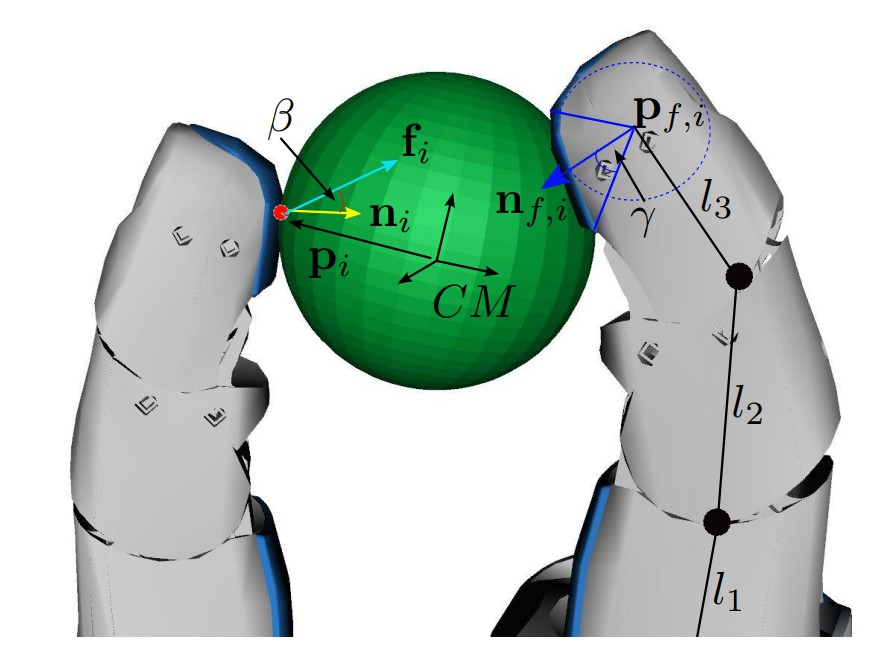
\includegraphics[width=0.98\hsize]{fig/1-introduction/Hertkorn/fig1.jpg}
\subcaption{The contact points}
\end{minipage}\hfill
\begin{minipage}{0.33\hsize}
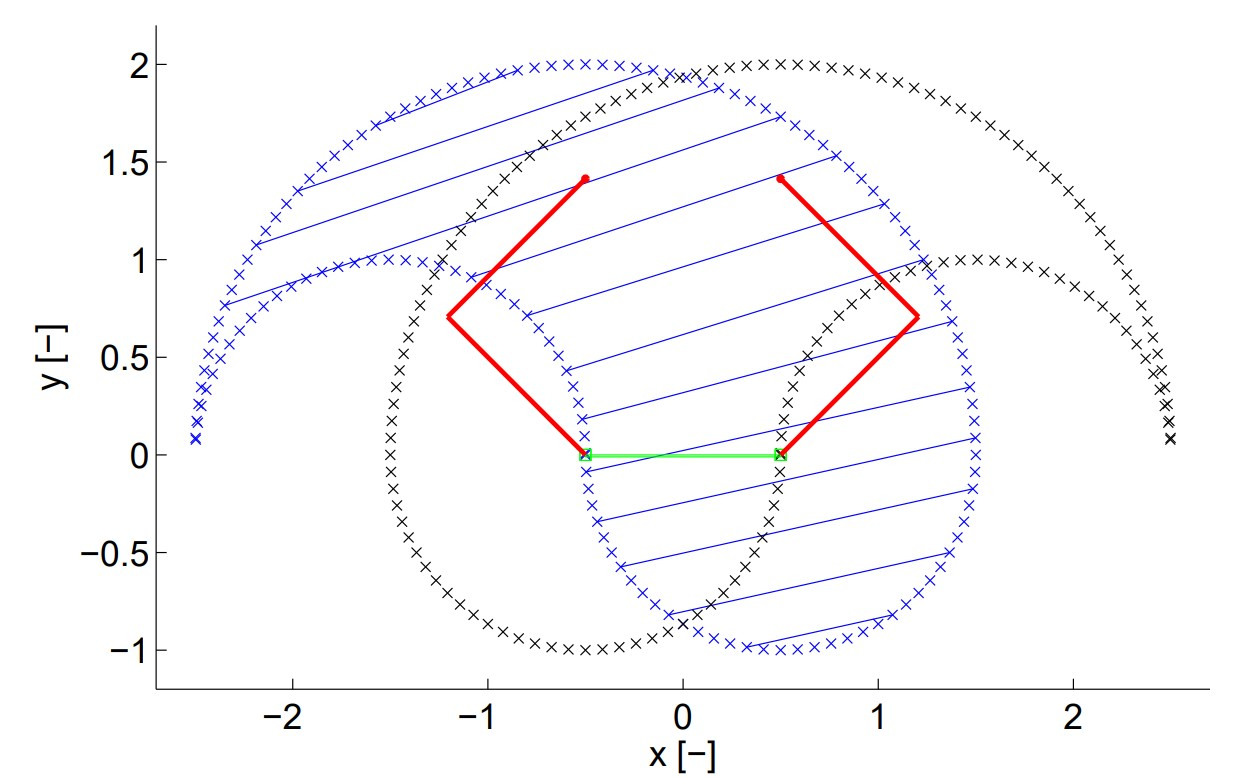
\includegraphics[width=0.98\hsize]{fig/1-introduction/Hertkorn/fig2.jpg}
\subcaption{The contact points}
\end{minipage}\hfill
\begin{minipage}{0.33\hsize}
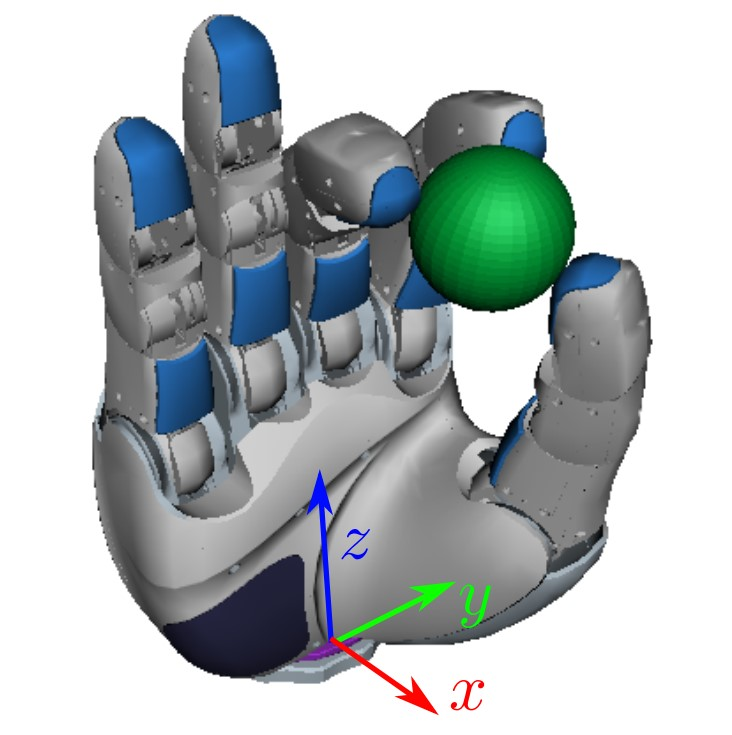
\includegraphics[width=0.98\hsize]{fig/1-introduction/Hertkorn/fig3.jpg}
\subcaption{The contact points}
\end{minipage}
\caption{Considered situation in \cite{hertkorn2013}}\label{fig::intro::hertkorn}
\end{figure}

\subsubsection{Energy Gradient-Based Graphs for Planning Within-Hand Caging Manipulation \cite{bircher2019}}
この研究では,ハンドと対象物からなる系のエネルギー情報を定義し,このエネルギーに基づいてマニピュレーション動作を決定している.
実験には,\figref{fig::system}のような劣駆動ハンドを用いており,アクチュエータへの2入力でハンドを制御している.エネルギー情報は,任意のアクチュエータ入力に対して,離散化空間内の全ての点のエネルギーを定義式より各々算出し,エネルギーマップを生成するという形で表現している.このエネルギーマップを様々なアクチュエータ入力に対して生成しておき,エネルギー勾配が対象物の目標座標へ向いているアクチュエータ入力を随時選び,ゴールを目指すといったアルゴリズムになっている.結果は,\figref{fig::manires}のようにマニピュレーションが実現されていた.

\begin{figure}[b]
	\centering
	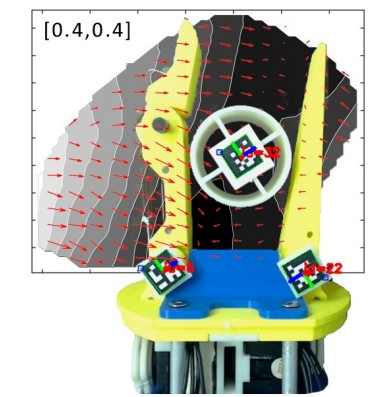
\includegraphics[width=0.3\hsize]{fig/1-introduction/bircher/handsystem.jpg}
	\caption{Robot system \cite{bircher2019}}
	\label{fig::system}
\end{figure}
\begin{figure}[b]
\centering
\begin{minipage}{0.24\hsize}
\centering
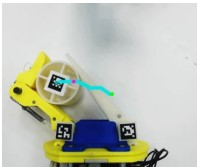
\includegraphics[width=\hsize]{fig/1-introduction/bircher/mani_a.jpg}
\subcaption{}
\end{minipage}
\begin{minipage}{0.24\hsize}
\centering
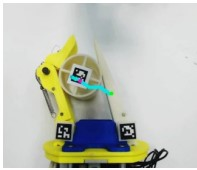
\includegraphics[width=\hsize]{fig/1-introduction/bircher/mani_b.jpg}
\subcaption{}
\end{minipage}	\hfill
\begin{minipage}{0.24\hsize}
\centering
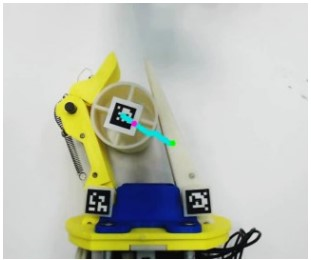
\includegraphics[width=\hsize]{fig/1-introduction/bircher/mani_c.jpg}
\subcaption{}
\end{minipage}	\hfill
\begin{minipage}{0.24\hsize}
\centering
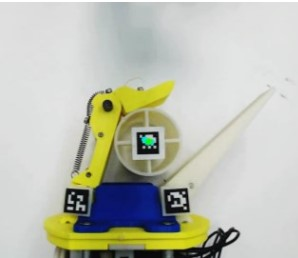
\includegraphics[width=\hsize]{fig/1-introduction/bircher/mani_d.jpg}
\subcaption{}
\end{minipage}	\hfill
\caption{Manipulation results \cite{bircher2019}}
\label{fig::manires}
\end{figure}

\subsubsection{Planar In-Hand Manipulation Via Motion Cones \cite{chavan-dafle2020}}
この研究では,\figref{fig::maniT}のようにグリッパで対象物を把持し,壁等の外部環境に押し付けたタイミングで把持位置をスライドさせることで持ち替え動作を行っている.ただし,動作計画ではグリッパが固定されており,壁等の環境がプッシャとして対象物を押し出すといった見方をしている.動作計画にあたって,Motion cone (動作円錐)というものを考えている.これは,摩擦の作用を考慮したうえで対象物が1プッシュで到達可能な領域を意味する.動作計画アルゴリズムにはT-RRT*を用いており,ランダムサンプリングしたノードが親ノードのMotion cone内でかつ,効率的な動きである場合,木構造に追加する.Motion cone外であった場合は,Motion cone内に投影した点を用いて同様の判定を行っていた.この手順で枝を伸ばしていき,目標状態となったとき計画を終了している.以上の動作計画のイメージを\figref{fig::rrtimage}に示している.上記の手法に基づき,数多くの実験検証を行い,理論が正確であることが確認されていた.
\begin{figure}
\begin{minipage}{0.49\hsize}
\centering
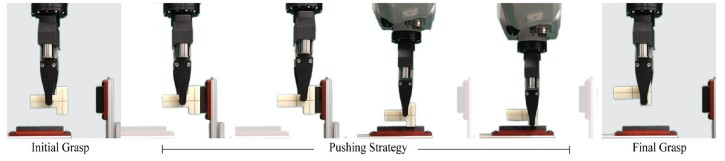
\includegraphics[width=0.9\hsize]{fig/1-introduction/chavan-dafle/manipulation.jpg}
\caption{Manipulating a T-shaped object in a parallel-jaw grasp by pushing it against features in the environment \cite{chavan-dafle2020}}
\label{fig::maniT}
\end{minipage} \hfill
\begin{minipage}{0.49\hsize}
\centering
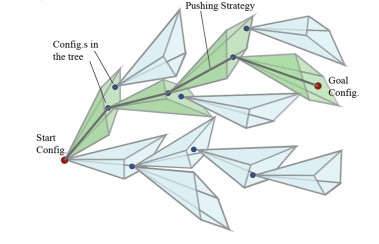
\includegraphics[width=0.8\hsize]{fig/1-introduction/chavan-dafle/rrtimage.jpg}
\caption{The image of motion planner \cite{chavan-dafle2020}}
\label{fig::rrtimage}
\end{minipage}
\end{figure}

\subsubsection{まとめ}
In-handマニピュレーションに取り組んだものを紹介した.これらの研究は,マニピュレーション中に対象物に関する力情報や位置情報を必要としており,センシングが不可欠となっている.


\subsection{センサレスなマニピュレーションを行っている研究}
\subsubsection{Sensorless In-Hand Manipulation by An Underactuated Robot Hand \cite{ospina2020}}	\label{sec::ospina}
この研究では,センサレスかつ対象物体の幾何情報なしのIn-handマニピュレーションを提案している.\figref{fig::ohand}のようなハンドを用いており,これは2つのリンクに対して1つのアクチュエータで駆動する劣駆動ハンドとなっている.このハンド先端の円形部分で物体を挟み込み,物体操りを行っている.センサレスなマニピュレーションを実現するため,全ての把持の状態を領域化した,In-hand Manipulability Region (IHMR)というものを定義している.IHMRの範囲内でハンドを動かす限り,把持が成立し続ける.IHMRは物体形状に依存するため,様々な既知物体に対してIHMRを算出し,それらの共通領域を任意物体のIHMRとすることで,幾何情報を必要としないセンサレスin-handマニピュレーションを実現していた.
\begin{figure}[b]
\begin{minipage}{0.49\hsize}
\centering
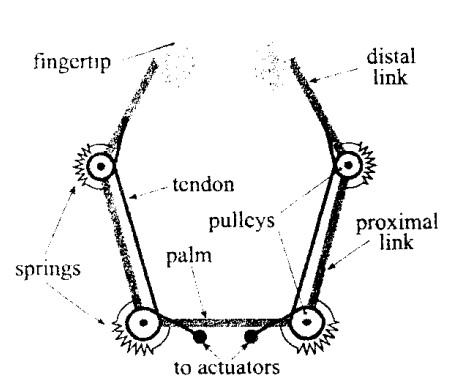
\includegraphics[width=0.9\hsize]{fig/1-introduction/Ospina/handmodel.jpg}
\caption{Two-finger underactuated hand \cite{ospina2020}}
\label{fig::ohand}
\end{minipage} \hfill
\begin{minipage}{0.49\hsize}
\centering
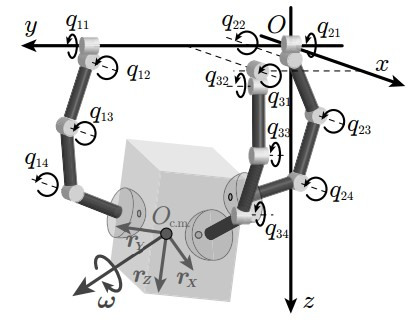
\includegraphics[width=0.9\hsize]{fig/1-introduction/tahara/modeling.jpg}
\caption{Grasping model with three-finger hand \cite{tahara2020}}
\label{fig::model}
\end{minipage}
\end{figure}


\subsubsection{動的安定把持に基づくマニピュレーション \cite{tahara2013}\\多指ロボットハンドによる物体把持のダイナミクスと受動性 \cite{tahara2020}}
この研究では「受動性」の概念を導入することで指が物体と接触している間についてのダイナミクスの特性を解析している.受動性とは簡単に言うと制御における安定性の指標であり,受動性を満たすとき可制御であるとは限らないが,少なくとも内部エネルギーが意図せず増加しない安定状態となっている.\figref{fig::model}のように指先を半球状のモデルで表現し,指先と物体間の接触点位置拘束と転がり速度拘束条件を考慮した運動方程式を立式していた.これに対し,系が受動性を満たすような制御入力を設計することで,安定した把持を実現していた.制御入力はロボットハンドの内界センサ値のみで算出される値であり,センサレスな把持が可能となっていた.

\subsubsection{Sensorless Pose Determination Using  Randomized Action Sequences ~\cite{mannam2019}}
本研究では,\figref{fig::trayrobot}のようにロボットの手先につけたトレーをランダムに何度も傾けることで,物体姿勢のばらつきを定量化したエントロピーを減少させることができることを提案・検証している.ランダムな動作の利点として,物体形状を考える必要がなく,システムが単純であることが挙げられている.実機での検証では,\figref{fig::entropy}のように全体的にみるとエントロピーが減少しており,センサレスで対象物の姿勢をある程度同定できることを示した.
\begin{figure}[t]
\begin{minipage}{0.49\hsize}
\centering
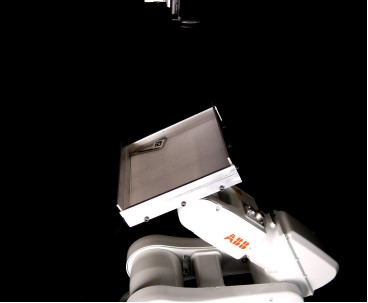
\includegraphics[width=0.9\hsize]{fig/1-introduction/Mannam/trayrobot.jpg}
\caption{An industrial robot with tray \cite{mannam2019}}
\label{fig::trayrobot}
\end{minipage}\hfill
\begin{minipage}{0.49\hsize}
\centering
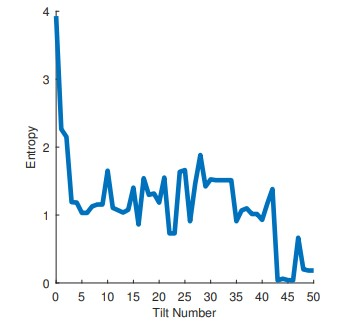
\includegraphics[width=0.9\hsize]{fig/1-introduction/Mannam/entropy.jpg}
\caption{Robot entropy data \cite{mannam2019}}
\label{fig::entropy}
\end{minipage}
\end{figure}

\subsubsection{まとめ}
これらの研究は,センサレスでマニピュレーションを行うという点で本研究グループのセンサレスin-handケージングマニピュレーションと類似している.しかし,以下の観点で本研究グループの手法の独自性・優位性が主張できる.
\cite{ospina2020}は義手への応用を見込んでおり,把持を維持することに重きを置いているため,把持物体を目標位置・姿勢へ精確に運ぶといったタスクには向かない.\cite{tahara2013}\cite{tahara2020}も同様に把持を安定させることに注力しており,物体の目標位置・姿勢への収束は別の議論が必要である.\cite{mannam2019}はセンサレスかつ物体形状に依存しない点から我々の手法より汎用性が高いと言える.しかし,整列に非常に長い時間がかかる.我々のようにパーツフィーダへの応用を前提としている場合,整列時間は生産効率を左右する重要な要素であり,整列時間に優位性があるのは大きなメリットである.


\subsection{パーツフィーダ研究・製品}
%従来のパーツフィーダシステムあったほうがいいかも
\begin{figure}[t]
\begin{minipage}{0.49\hsize}
\centering
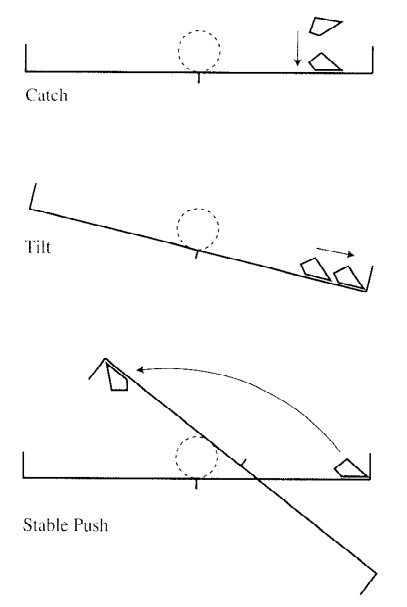
\includegraphics[width=0.9\hsize]{fig/1-introduction/Akella/sensorless_movement.jpg}
\caption{Primitives used for sensorless orienting \cite{akella2000}}
\label{fig::sensmov}
\end{minipage}
\begin{minipage}{0.5\hsize}
\centering
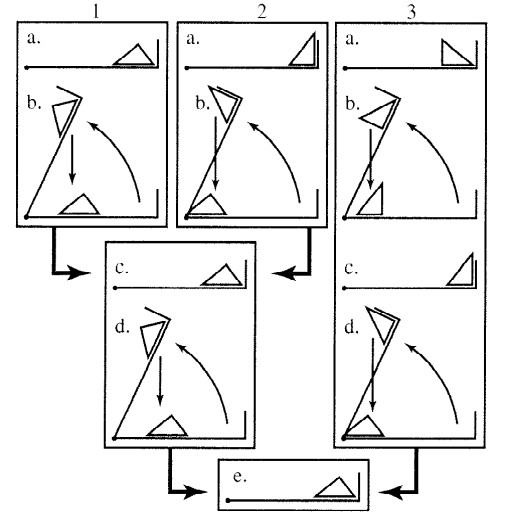
\includegraphics[width=0.9\hsize]{fig/1-introduction/Akella/sensorless_result.jpg}
\caption{Example sensorless feeding plans for a triangle \cite{akella2000}}
\label{fig::sensres}
\end{minipage}

\centering
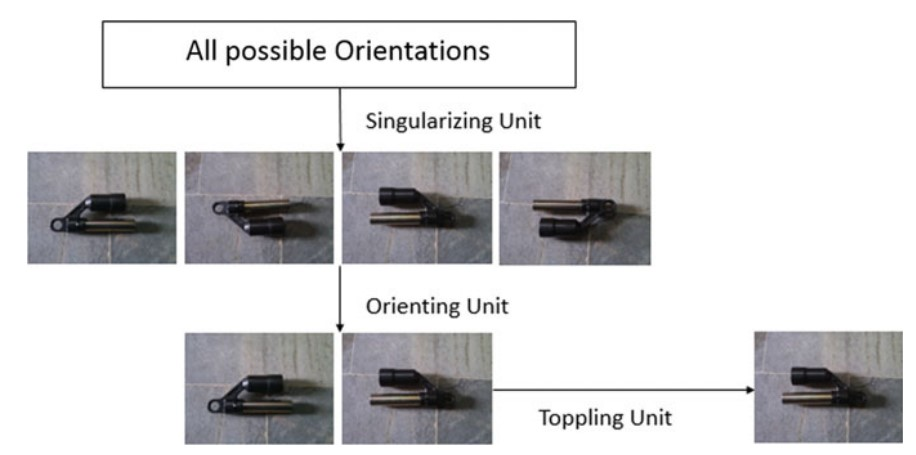
\includegraphics[width=0.6\hsize]{fig/1-introduction/Udhayakumar/threephase.jpg}
\caption{Three phases of orientation \cite{Udhayakumar}}
\label{fig::three}

\end{figure}
\subsubsection{Parts Feeding on a Conveyor with a One Joint Robot \cite{akella2000}}
この研究では,一つの関節のみを持つロボットとベルトコンベアのみを用いてセンサレスで物体操作を行っている.
\figref{fig::sensmov}の3つの動作のみを用いており,catch動作で対象物の辺をハンドに接触させるところから始まり,物体を目標姿勢へ遷移させることができるような動作組み合わせを計算している.動作例は\figref{fig::sensres}のようになっており,異なる初期状態の対象物に対して同じ目標姿勢へと遷移させていた.
%限界は,凸多角形以外の場合は難しいことが多い,姿勢のみしか整列できない,摩擦なしを仮定,


\subsubsection{Development of Visionless Flexible Part Feeder for Handling Shock Absorbers \cite{udhayakumar2021}}
この研究では,パーツフィーダの設計・製作から行う安価なシステムを提案している.shock absorberの部品に対象を絞り,次の3手順(\figref{fig::three}),(1) Singularizing Unit,(2) Orienting Unit, (3) Toppling Unit,を順に行い整列していた.(1)は物体を水平方向へ整列させるタスク,(2)は近接センサで上下判定を行い,下向きの場合に上向きに反転させるタスク,(3)は近接センサで左右の向きを検知し,目標姿勢ではない場合は部品を反転させるタスクである.このように,各手順で物体の取りうる姿勢を減らしていくことで,最終的に一つの目標姿勢へと遷移させていた


\subsubsection{まとめ}
\cite{akella2000},\cite{udhayakumar2021}は,物体操作を用いてパーツフィーダを開発している研究である.前者の研究は姿勢のみしか整列できないことが,後者は部品の汎用性がないことがそれぞれ課題点となっている.

\subsection{本研究室の従来研究}
本研究室では,「センサレスin-handケージングマニピュレーション」というマニピュレーション手法を提案している.力覚センサを必要とせずハンドの位置制御のみで対象物を拘束できるケージングという考え方を応用することで,対象物を「センサレス」に目標点までマニピュレーションすることができる.
また,ハンド構成に十分な自由度を持たせていることにより,多様な形状の対象物を取り扱えるといった特徴もある.
本手法は,位置・姿勢にばらつきのある対象物を目標の位置・姿勢へと遷移させられるといった特徴から,工場の製造ライン等で乱雑に流れてくる部品を整列させるパーツフィーダへ応用できる.

\subsubsection{センサレスin-handケージングマニピュレーションによる物体の位置・姿勢制御 \cite{komiyama2021}}
以前の研究\cite{asamura2013}では,マニピュレーションにおいて位置の整列のみ行われており,姿勢は考慮されていなかった.それゆえ,円形物体しか取り扱えていなかった.そこで,\cite{komiyama2021}は位置と姿勢の両方を取り扱う手法を提案し,三角形,長方形,L字型等の多様な形状の対象物を取り扱えるようにした.
6自由度ハンドを用いて,上記の対象物に対してマニピュレーションされることを確認していた(\figref{fig::intro::recmani}).


\subsubsection{センサレスin-handケージングマニピュレーションに基づく汎用パーツフィーダの開発 \cite{kamikukita2022}}
この研究では,センサレスin-handケージングマニピュレーションという手法を基に,ベルトコンベアと従来のハンドを用いた汎用パーツフィーダが開発された.ベルトコンベアにより流れてきた対象物に対して,ハンドでキャッチ,マニピュレーション,リリースという一連の動作でパーツフィーダとしての機能を実現していた(\figref{fig::intro::trimani}).また,本手法では180$^\circ$程度の大回転が難しいといった問題点があったが,ベルトコンベアの正転・逆転を利用し,実現していた.
\begin{figure}[b]
\begin{minipage}{0.24\hsize}
\centering
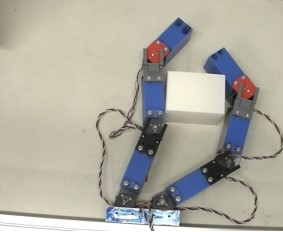
\includegraphics[width=\hsize]{fig/1-introduction/mani1.jpg}
\subcaption{}
\end{minipage}\hfill
\begin{minipage}{0.24\hsize}
\centering
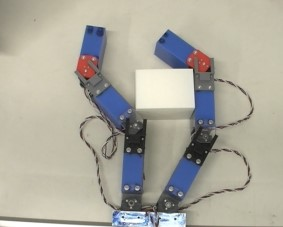
\includegraphics[width=\hsize]{fig/1-introduction/mani2.jpg}
\subcaption{}
\end{minipage}\hfill
\begin{minipage}{0.24\hsize}
\centering
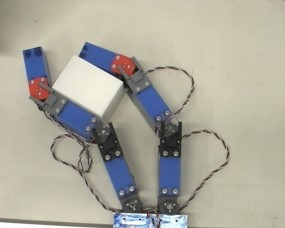
\includegraphics[width=\hsize]{fig/1-introduction/mani3.jpg}
\subcaption{}
\end{minipage}\hfill
\begin{minipage}{0.24\hsize}
\centering
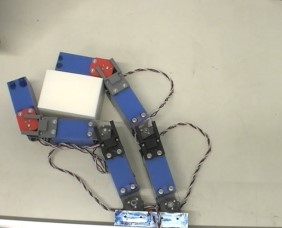
\includegraphics[width=\hsize]{fig/1-introduction/mani4.jpg}
\subcaption{}
\end{minipage}
\caption{Rectangle manipulation \cite{komiyama2021}}
\label{fig::intro::recmani}

\begin{minipage}{0.49\hsize}
\centering
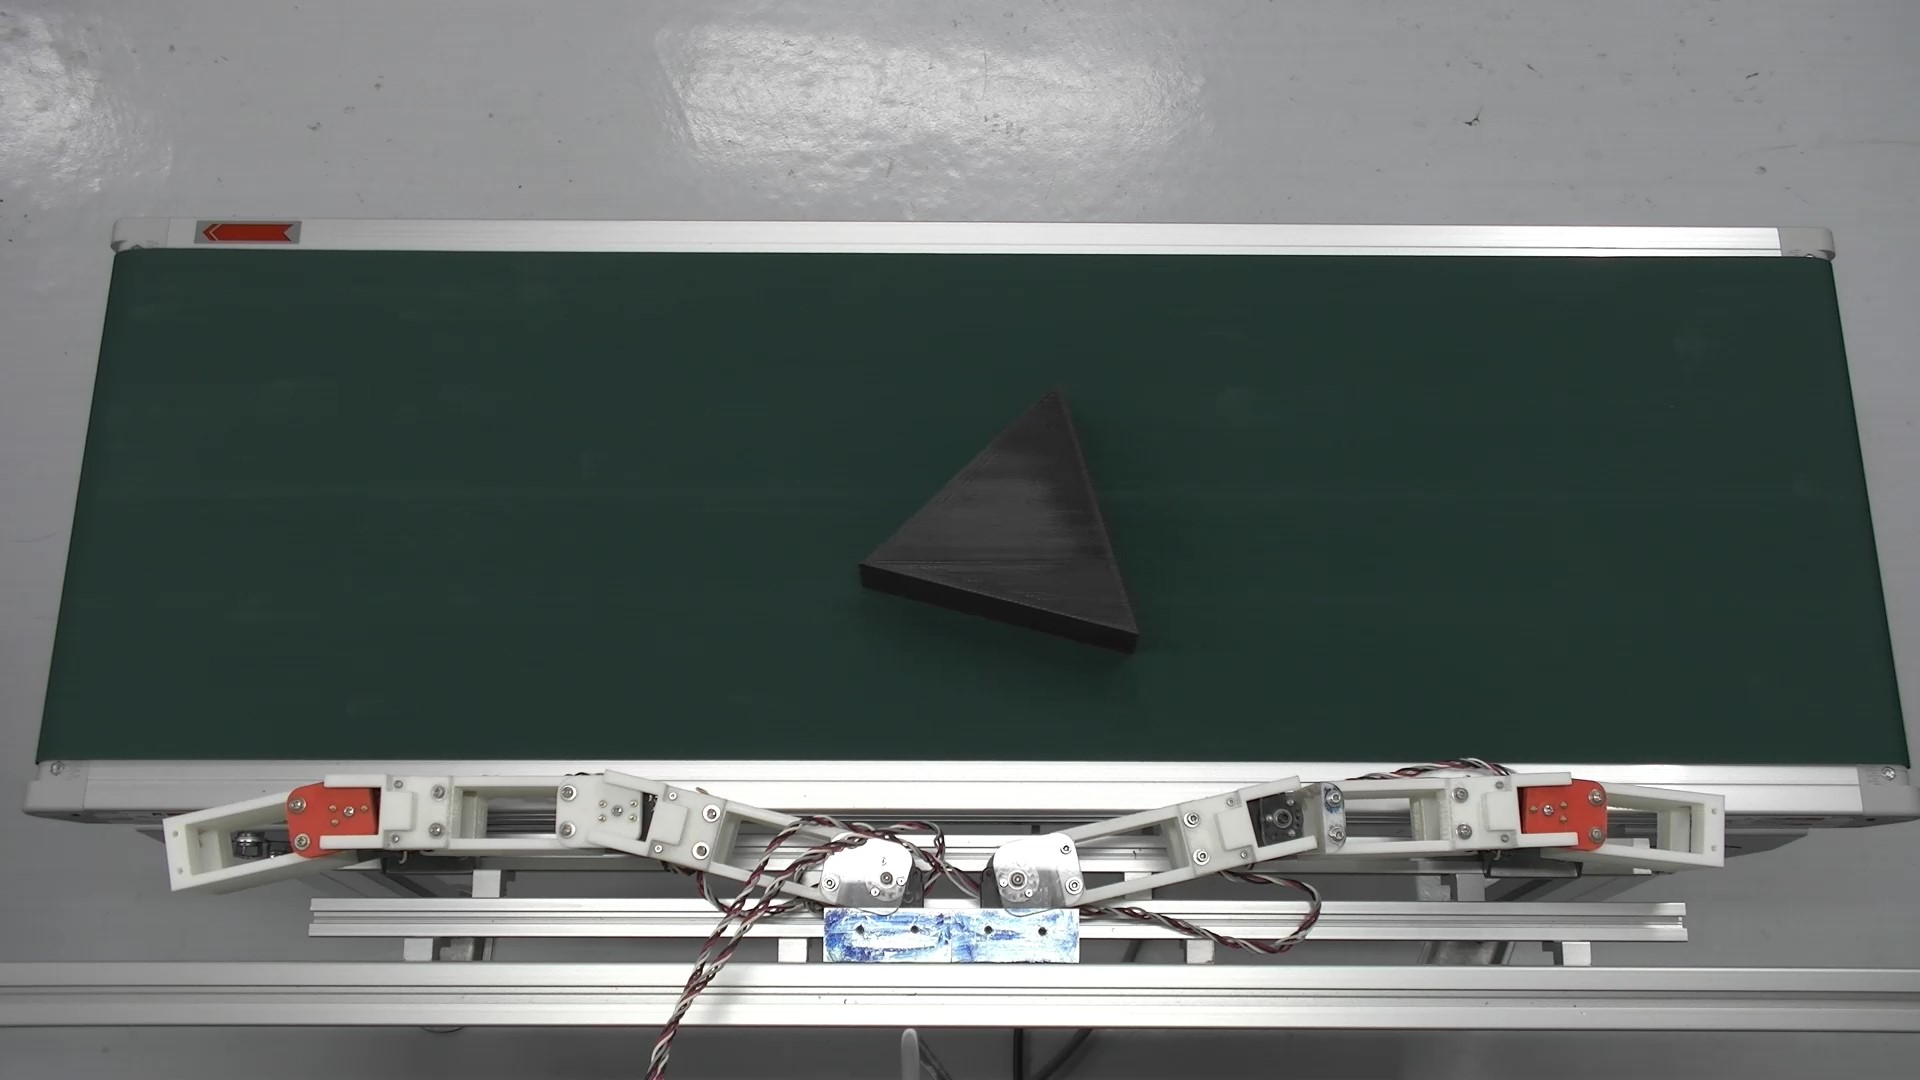
\includegraphics[width=\hsize]{fig/1-introduction/triangle_Moment_2.jpg}
\subcaption{}
\end{minipage}\hfill
\begin{minipage}{0.49\hsize}
\centering
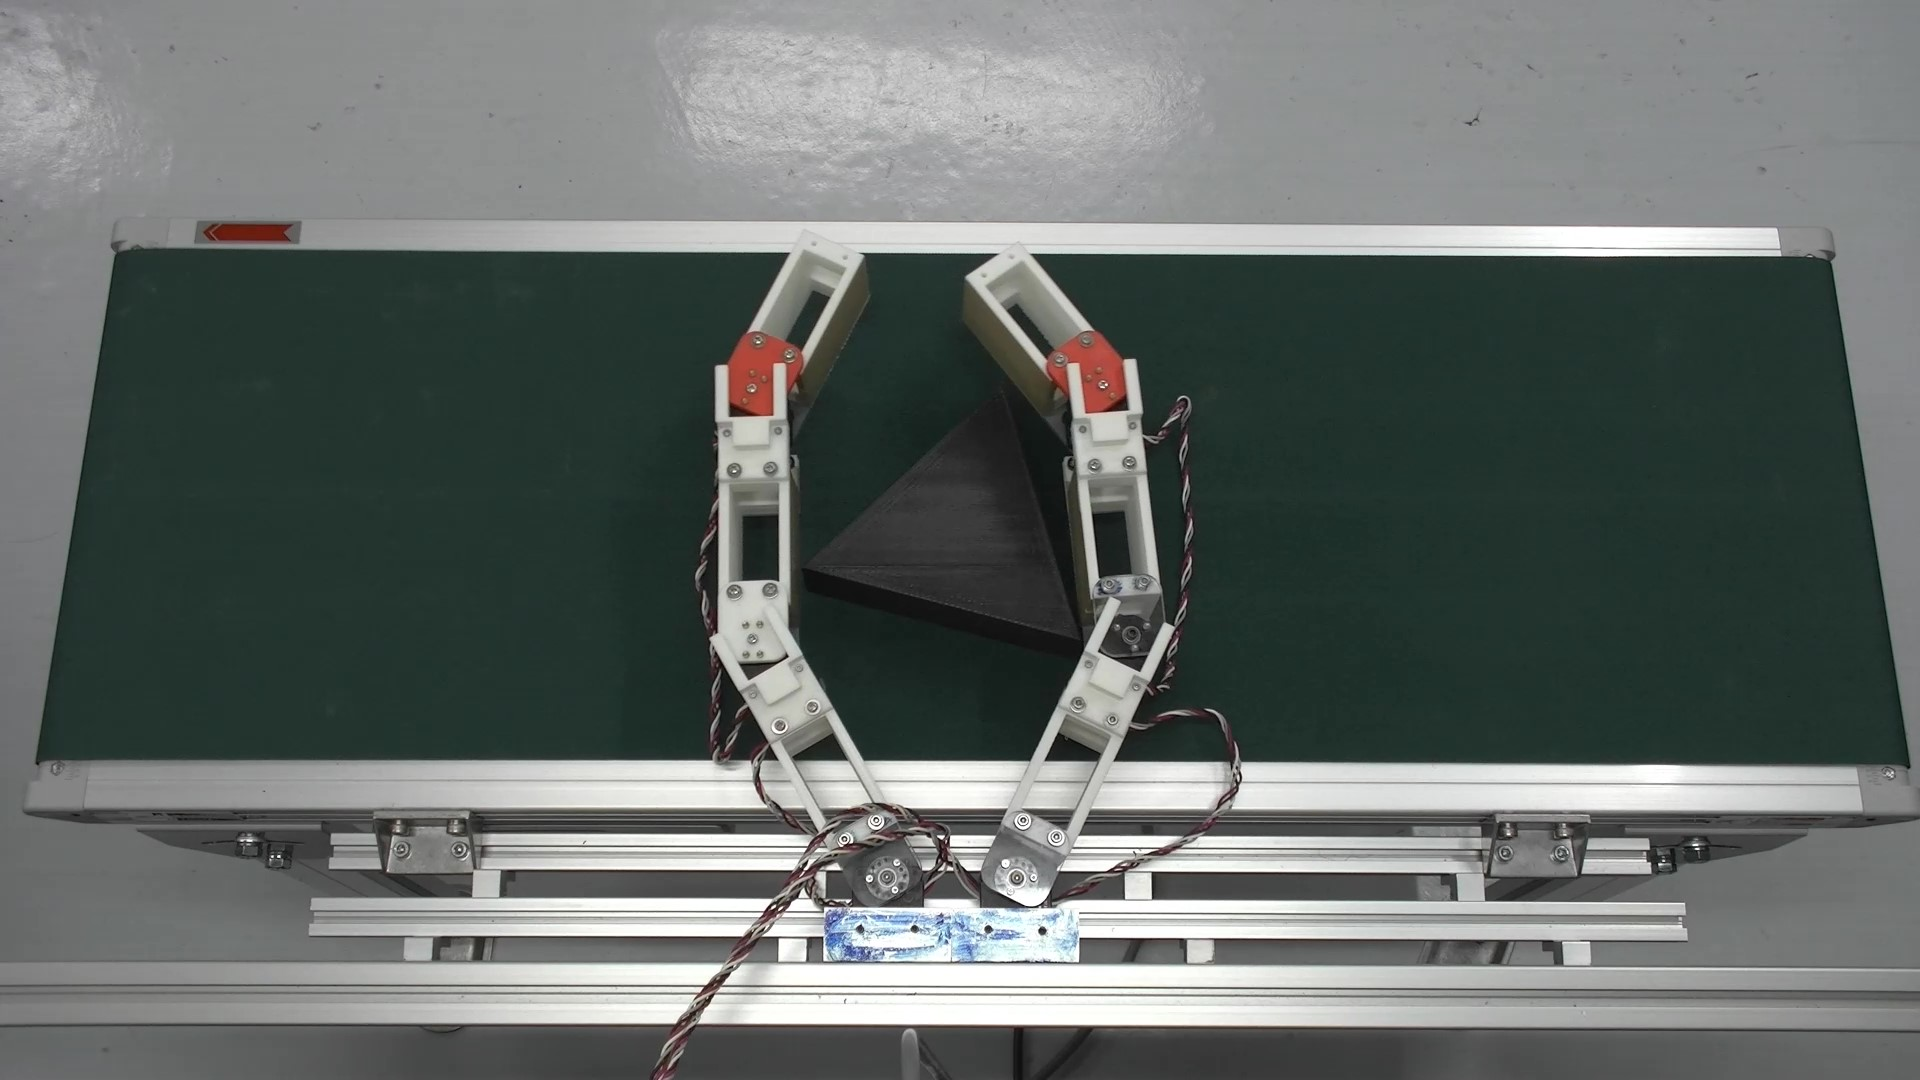
\includegraphics[width=\hsize]{fig/1-introduction/triangle_Moment_3.jpg}
\subcaption{}
\end{minipage}\\
\begin{minipage}{0.49\hsize}
\centering
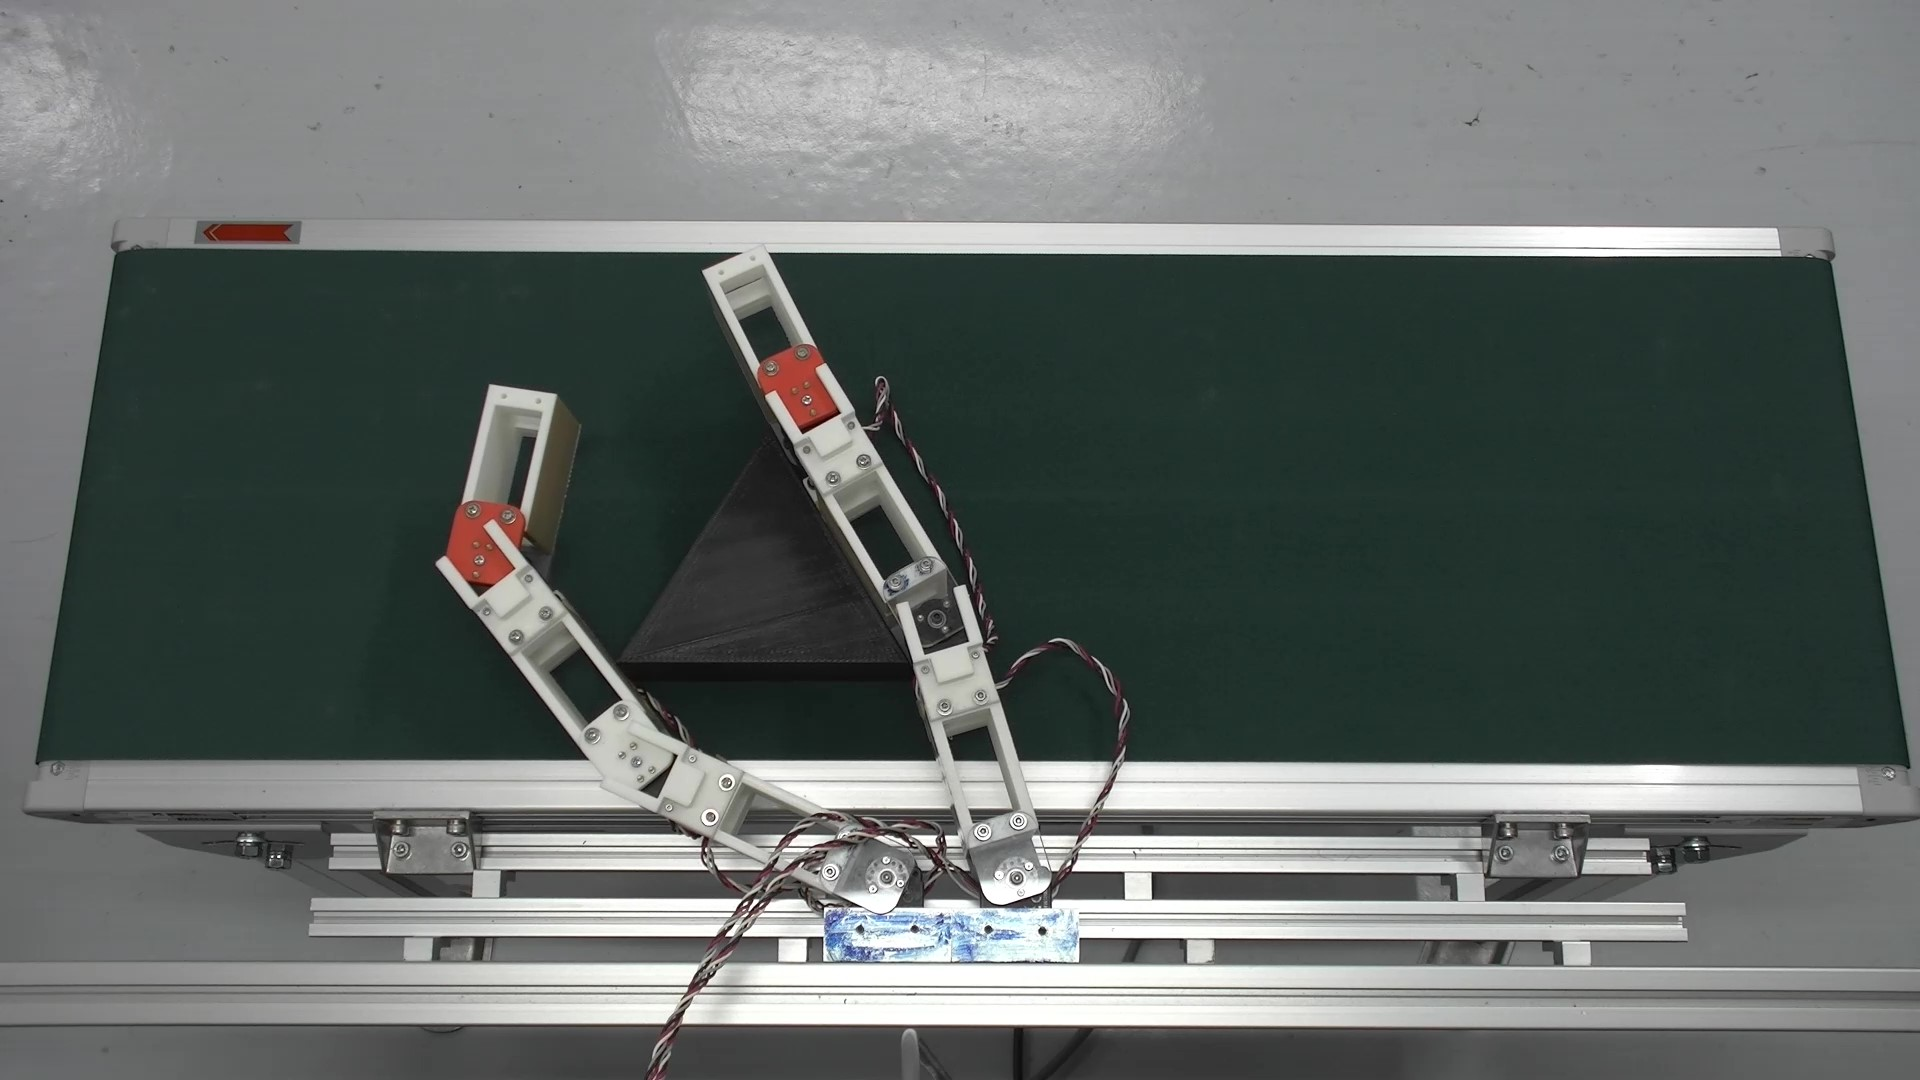
\includegraphics[width=\hsize]{fig/1-introduction/triangle_Moment_5.jpg}
\subcaption{}
\end{minipage}\hfill
\begin{minipage}{0.49\hsize}
\centering
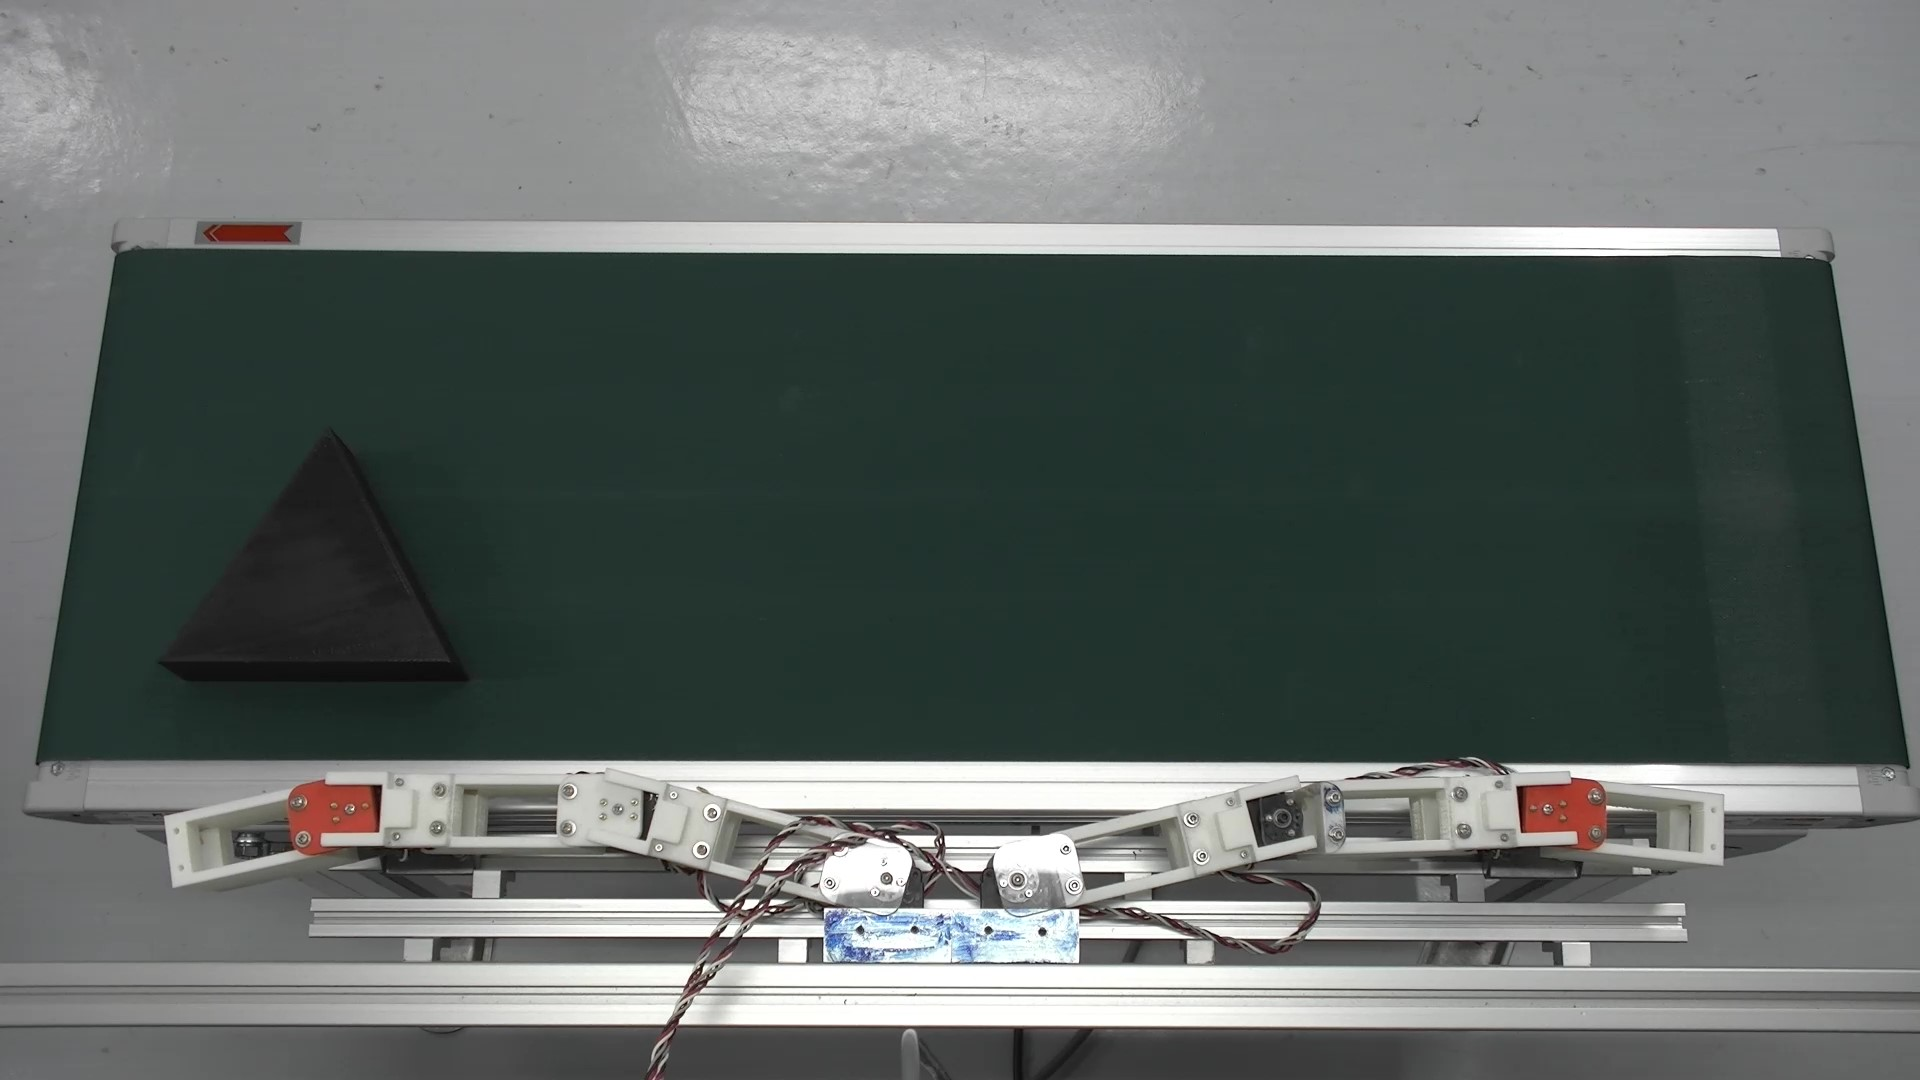
\includegraphics[width=\hsize]{fig/1-introduction/triangle_Moment_7.jpg}
\subcaption{}
\end{minipage}
\caption{Triangle manipulation as part feeder \cite{kamikukita2022}}
\label{fig::intro::trimani}
\end{figure}

\section{研究目的}\label{sec::intro::objective}
\cite{komiyama2021}で,センサレスin-handケージングマニピュレーションにおいて実現したい機能は実装された.しかし,パーツフィーダとしての実用化を目指す上で,以下の課題が存在する.1つ目に対象物がハンドに詰まり,正常にハンドを動かせなくなる「ジャミング」が起きる点,2つ目にハンド動作計画の計算時間が長くかかる点,そして3つ目に対象物の位置決め精度が十分ではないという点である.\par

1つ目に関して,ジャミングは\cite{asamura2013}から存在するセンサレスin-handケージングマニピュレーションの課題である.\cite{komiyama2021}では,ヒューリスティクス的なアプローチで解決を試みた.これにより,ある程度はジャミングを回避できるようになったが,全ての場合に対応できるわけではなく,依然としてジャミングは起こっていた.\cite{kamikukita2022}では,ジャミング時にベルトコンベアを回すことで対象物の状態を変化させ,解消する試みがなされた.この操作を時には複数回繰り返すことで,多くの場合でジャミングを回避できるようになったが,繰り返し操作分,整列時間が長くかかっていた.本手法はパーツフィーダへの応用を見込んでいるので,整列時間の増加は生産効率の低下につながり,望ましくない.

2つ目の計算時間に関しては,一つの動作計画を生成するのに短くとも数時間,長いと数日を要していた.また,3つ目の位置決めは精度に関して,\cite{komiyama2021}では動作計画時で位置誤差が最大20[mm],姿勢誤差が最大20[deg]生じ得ており,実機の場合はそれ以上の誤差が発生していた.実機精度の向上も必要だが,動作計画の理論計算においてこれほどの誤差が出るのは問題である.本研究においては動作計画での位置決め精度向上を主に取り組む.

2つ目と3つ目の課題はどちらも動作計画に関する課題である.これらの課題は互いに関連しており,計算時間を抑えようとすると位置決め精度が悪くなり,位置決め精度を上げようとすると計算時間が長くなるという関係にある.

そこで,本論文ではこれらの改善に取り組むべく,以下の2点を目標として掲げる.
\begin{itemize}
\item ジャミングの回避
\item 動作計画の計算時間と位置決め精度の総合的な性能向上
\end{itemize}
これにより,センサレスin-handケージングマニピュレーションの有用性が高まり,整列時間,再立ち上げ時間が短く,位置決め精度も高い,パーツフィーダの開発に貢献できると考えている.

\section{本論文の構成}\label{sec::intro::configuration}
本論文の構成を以下に示す.\par
本章では,研究の背景,従来研究について述べ,研究の目的を「ジャミングの回避」,「動作計画の計算時間と位置決め精度の総合的な性能向上」の2つに定めた.\par
2章では,本研究室で提案されてきた平面内センサレスin-handケージングマニピュレーションについて述べる.\par
3章では,従来の動作計画の改良点と新たな動作計画手法について述べる.\par
4章では,提案手法を用いた多角形物体の平面内センサレスin-handケージングマニピュレーションの計画および実機による検証について述べる.\par
5章では,本研究の結論と今後の展望について述べる.


% 白魔術
\expandafter\ifx\csname ifdraft\endcsname\relax
    \end{document}
\fi
